\subsection{毛管波：PhaseRegion graph chart の正規ルート}
\label{sec:val_capillary}
% ═══════════════════════════════════════════════════════════════════

\subsubsection{設定と理論基準}

毛管波ベンチマークは，平坦界面に小振幅の正弦波摂動を与え，
表面張力による復元振動を観察する最も単純な移動界面テストである．
本節では，旧 production runtime の速度・圧力可視化ではなく，
第~\ref{sec:ao_fast_state_space}節で導いた PhaseRegion 正規経路を
標準の入口として用いる．
すなわち，所有者は
\[
  \Omega_g(t)=\{y>\eta(x,t)\},
  \qquad
  \Gamma_h(t)=\partial\Omega_g(t)
\]
であり，セル測度は $q_g=Q_h(\Omega_g)$，
液相測度は $q_l=|C|-q_g$ として従属的に読む．
$\eta$ は graph chart，$\phi$ は必要なら作る gauge であり，
どちらも単独では物理状態の所有者ではない．

初期界面は
\begin{equation}
  y_\Gamma(x,0)=y_0 + A_0\cos(kx+\theta_0),
  \qquad
  k=\frac{2\pi m}{L_x}.
  \label{eq:capillary_wave_initial}
\end{equation}
初期条件は水--空気の実スケールとして
$y_0=0.01\,\mathrm{m}$，$A_0=2.0\times10^{-4}\,\mathrm{m}$，
$m=2$，$L_x=0.02\,\mathrm{m}$，$\theta_0=0$ とする．
上下壁の間に置かれた有限深さ二流体の小振幅理論では
\begin{equation}
  \omega^2
  = \frac{\sigma k^3}
         {\rho_l\coth(kh_l)+\rho_g\coth(kh_g)},
  \qquad
  h_l=h_g=0.01\,\mathrm{m},\quad g=0,
  \label{eq:flat_capillary_dispersion}
\end{equation}
を位相基準に置く~\cite{Prosperetti1981}．
本設定では
\[
  \omega_\sigma
  =134.419859151\,\mathrm{s^{-1}},\qquad
  T_\sigma=\frac{2\pi}{\omega_\sigma}=0.046742983863\,\mathrm{s}
\]
である．

離散 route は次である：
\[
  \eta
  \longrightarrow
  q_l=Q_h(\eta)
  \longrightarrow
  q_g=|C|-q_l
  \longrightarrow
  \mathrm{PhaseRegionBatch}(\mathrm{GAS\_ABOVE},\mathrm{graph})
  \longrightarrow
  E_h^{(2)}[\eta].
\]
$Q_h$ は列ごとの exact P1 graph column-integral で評価し，
$E_h^{(2)}$ は同じ graph perimeter の二次変分として
線形毛管波 mode を進める．
時間発展は velocity-Verlet の reduced chart stepper であり，
圧力・速度場へ PhaseRegion face force を消費する段階は未接続である．
したがって本節の合格条件は，厳密解との振幅・速度・エネルギー比較，
$Q_h$ 測度残差，体積ドリフト，GPU hot path，および
\texttt{force\_admissible=0} の fail-close である．

\begin{itemize}[noitemsep,leftmargin=2em]
  \item 正規入口：\texttt{experiment/ch14/config/ch14\_capillary.yaml}
  \item 実行：\texttt{experiment/ch14/diagnose\_phase\_region\_capillary\_graph\_steps.py}
  \item グリッド：$[0,0.02]^2\,\mathrm{m}^2$，$32^2$，
        $x$ 周期，$y$ 壁面，legacy runtime YAML から読み込む診断格子
  \item PhaseRegion owner：\texttt{gas\_above}
  \item PhaseRegion chart：\texttt{graph\_periodic}
  \item PhaseRegion measurement：
        \texttt{exact\_graph\_column\_integral}
  \item 時間：$T=T_\sigma=0.046742983863\,\mathrm{s}$，
        $2560$ step，$\Delta t=1.825897807156\times10^{-5}\,\mathrm{s}$
  \item GPU：\texttt{backend.use\_gpu=true}，
        測度 reduction と owner map は \texttt{backend.xp} 上で実行
\end{itemize}

\subsubsection{結果と判定}

正規 YAML \texttt{ch14\_capillary.yaml} による 1 周期計算は，
remote GPU hot path で PASS した．
結果は表~\ref{tab:ch14_phase_region_capillary_graph} に示す．
終端時刻は $T_\sigma$ と一致し，
終端振幅 $1.999999999998\times10^{-4}\,\mathrm{m}$ は
厳密基準 $2.0\times10^{-4}\,\mathrm{m}$ と
$2.42\times10^{-10}\,\mathrm{m}$ 以下の最大誤差で一致した．
測度残差は全時刻で 0，体積ドリフトは
$5.43\times10^{-20}$ 以下である．
平均 step 時間は $3.52\times10^{-3}\,\mathrm{s}$，
最大 step 時間は $3.98\times10^{-2}\,\mathrm{s}$ であり，
$0.2\,\mathrm{s/step}$ の GPU 目標を満たした．

\begin{table}[!htbp]
\caption{N=32，PhaseRegion graph route 毛管波 1 周期計算}
\label{tab:ch14_phase_region_capillary_graph}
\centering\small
\begin{tabular}{lr}
\toprule
診断 & 値 \\
\midrule
steps & $2560$ \\
$t_{\mathrm{final}}/T_\sigma$ & $1.000000000000$ \\
\texttt{step\_backend\_gpu} & $1$ \\
\texttt{q\_measurement\_fast\_column\_integral} & $1$ \\
\texttt{max\_amplitude\_error} & $2.416836235604\times10^{-10}$ \\
\texttt{max\_velocity\_error} & $4.456387104473\times10^{-8}$ \\
\texttt{max\_energy\_drift} & $1.505982113082\times10^{-6}$ \\
\texttt{max\_residual\_l2} & $0$ \\
\texttt{max\_volume\_drift} & $5.421010862428\times10^{-20}$ \\
\texttt{mean\_step\_wall\_seconds} & $3.516834525792\times10^{-3}$ \\
\texttt{max\_step\_wall\_seconds} & $3.977783117443\times10^{-2}$ \\
\texttt{target\_met} & $1$ \\
\texttt{force\_admissible} & $0$ \\
\bottomrule
\end{tabular}
\end{table}

\begin{figure}[!htbp]
\centering
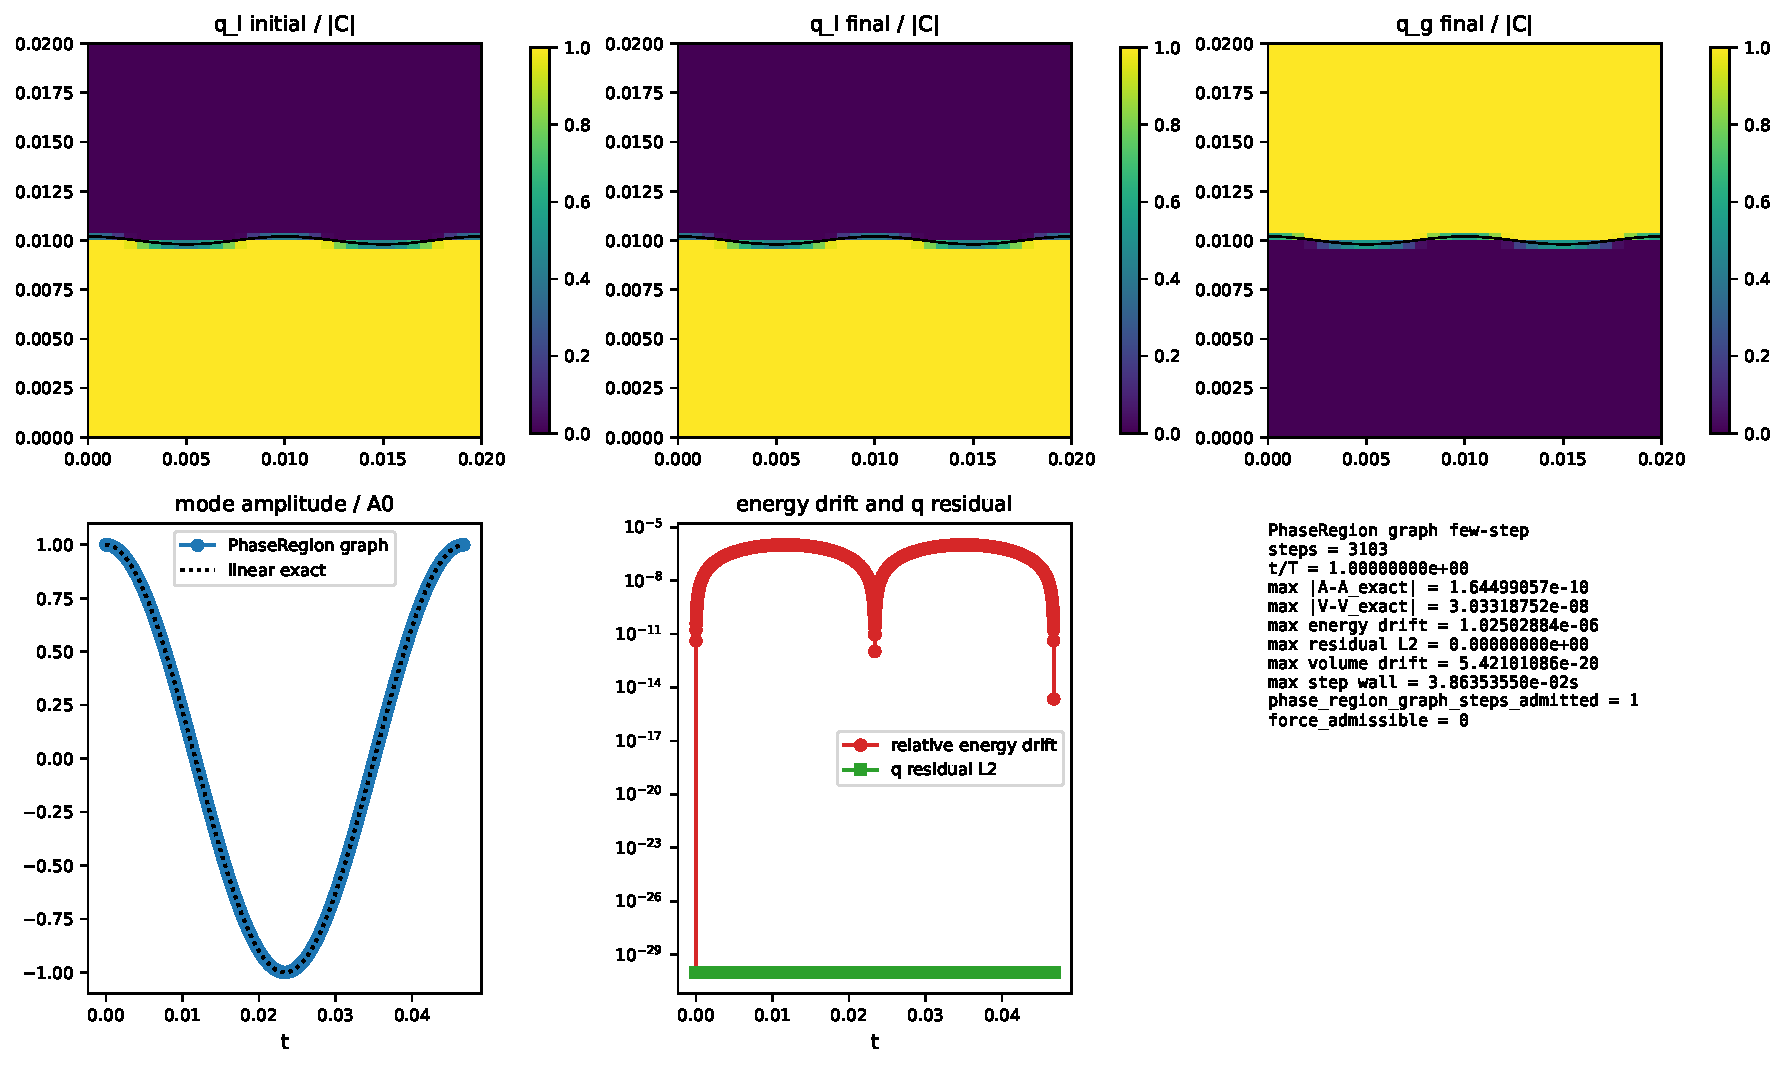
\includegraphics[width=0.92\linewidth]{figures/ch14_phase_region_capillary_graph_steps.pdf}
\caption{PhaseRegion graph route による N=32 毛管波 1 周期診断．
graph chart から作る $Q_h(\Omega_g)$，振幅の厳密解比較，エネルギー drift，
測度残差，体積 drift，および GPU step 時間を同じ reduced route 上で示す．}
\label{fig:ch14_phase_region_capillary_graph_steps}
\end{figure}

この結果の判定は，
「PhaseRegion が界面を所有し，$q$ は測度，
$\phi/\eta$ は chart である」という第~\ref{sec:ao_fast_state_space}節の
状態所有者が，毛管波 graph chart では可視化つきで動作した，
である．
重要なのは，これは旧 screened graph-$q$ projection の修理ではない点である．
旧経路では，輸送後の $q_T$ を滑らかな graph/phi chart に厳密に戻すことを
本体にしていたため，非幾何的なセル自由度を曲率へ押し付けた．
本節の正規 route は，$\Omega_g$ から $Q_h$ と $E_h$ を同時に読み，
測度残差を 0 として確認する reduced chart 問題である．

一方で，圧力・速度場はまだこの route の claim ではない．
PhaseRegion face cochain を production PPE/corrector へ消費する契約は
別ゲートであり，本節では \texttt{force\_admissible=0} を
明示したまま合格とする．
したがって旧 production runtime で生成された速度場・圧力場スナップショットは，
本節の PhaseRegion 正規ルートの成功根拠からは外す．

% ═══════════════════════════════════════════════════════════════════
